\documentclass{article}
\usepackage[utf8]{inputenc}
\usepackage{hyperref}
\usepackage{float}
\usepackage{graphicx}
\usepackage{caption}
\usepackage{subcaption}
\graphicspath{{./images/}}

\title{Super Mario World AI}
\author{Siebren Cosijn}
\begin{document}
    \maketitle

    \section{Introduction}
    \begin{figure}[H]
        \centering
        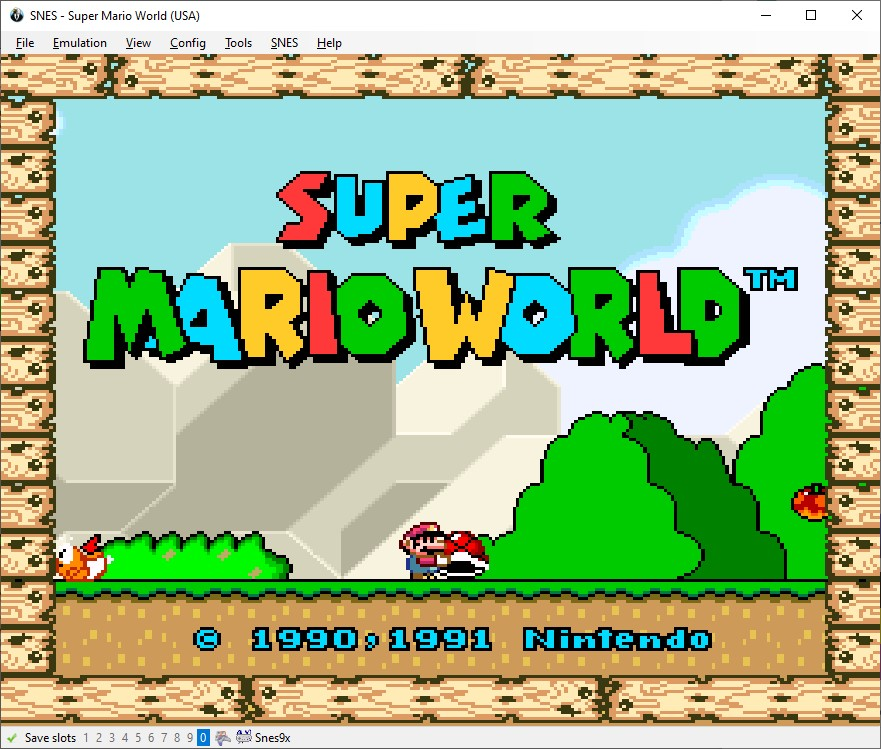
\includegraphics[width=0.85\textwidth]{start-screen}
    \end{figure}
    \begin{itemize}
        \item Super Mario World (SNES)
        \item Reinforcement learning
        \item OpenAI Gym\footnote{\url{https://github.com/openai/gym}} - RL library
        \item Gym Retro\footnote{\url{https://github.com/openai/retro/}} - Game integration for Gym
    \end{itemize}
    Reinforcement learning loop
    \begin{figure}[H]
        \centering
        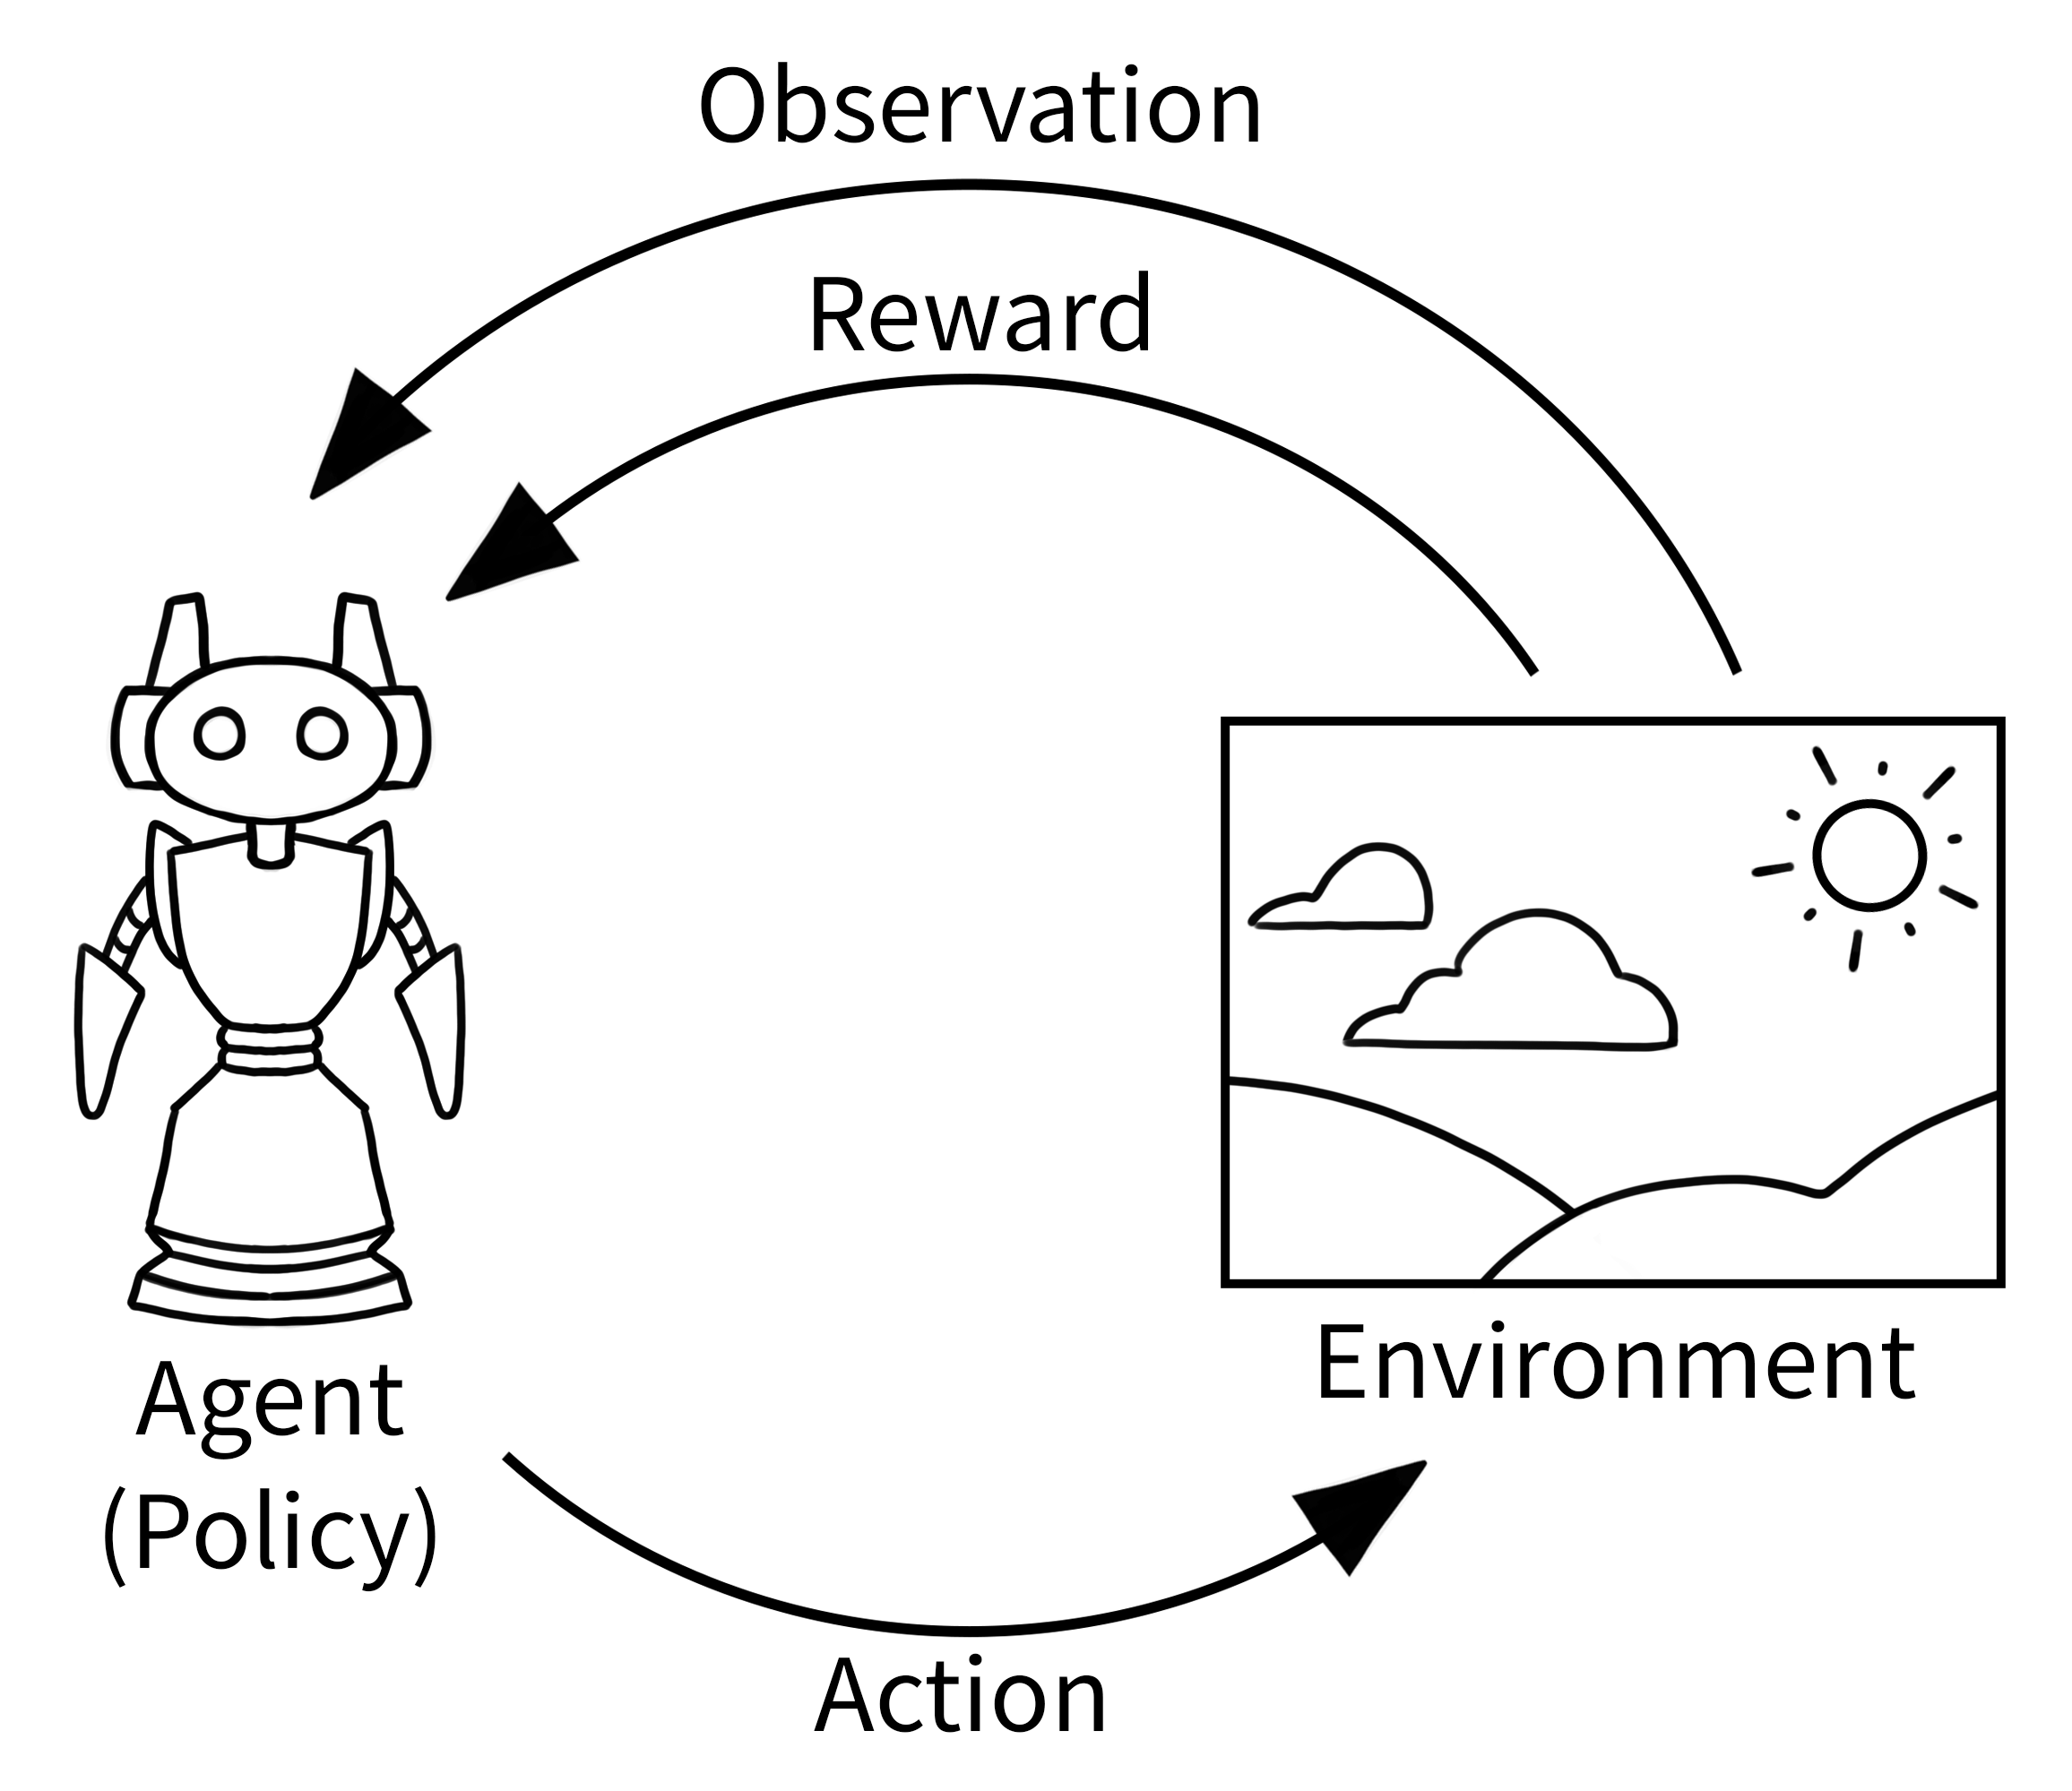
\includegraphics[width=0.65\textwidth]{AE_loop}
        \caption{\textbf{Source:} \url{https://www.gymlibrary.ml/_images/AE_loop.png}}
        \label{fig:loop}
    \end{figure}
    \begin{itemize}
        \item agent = RL model
        \item environment = game
        \item action = button input
        \item state = current frame
        \item reward = decide if action was good
    \end{itemize}

    \section{Goals}
    \begin{itemize}
        \item Train an agent to complete level(s) of the game
        \item Test agent on unseen levels
    \end{itemize}

    \section{Preprocessing}
    Based on 'Revisiting the Arcade Learning Environment'.
    Wrappers around the Gym environment.
    \subsection{Action Space}
    \begin{itemize}
        \item movement keys: none, left, right, down, up
        \item special keys: none, A (spin), B (jump), X = Y (run)
        \item multi-discrete space (max 1 of each)
        \item $5*4=20$ actions
    \end{itemize}
    \begin{figure}[H]
        \centering
        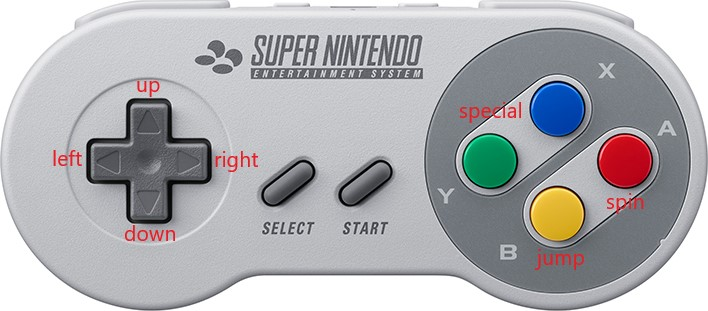
\includegraphics[width=.85\textwidth]{snes-controller-annot}
    \end{figure}
    \subsection{Observation Space}
    \subsubsection{Transform observation}
    \begin{itemize}
        \item 84x84 pixels
        \item Grayscale
        \item Reduced memory requirement
    \end{itemize}
    %TODO fix axes
    \begin{figure}[H]
        \centering
        \begin{subfigure}{.5\textwidth}
            \centering
            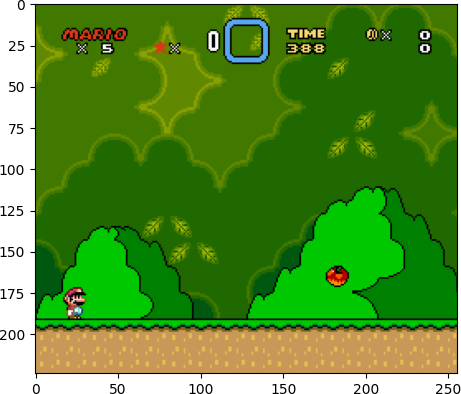
\includegraphics[height=5cm]{original_crop}
            \caption{Original}
            \label{fig:sub1}
        \end{subfigure}%
        \begin{subfigure}{.5\textwidth}
            \centering
            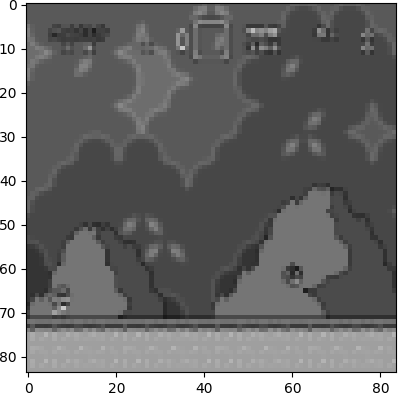
\includegraphics[height=3cm]{grayscale_crop}
            \caption{Transformed}
            \label{fig:sub2}
        \end{subfigure}
        \caption{Pixel Transformation}
        \label{fig:transformation}
    \end{figure}
    \subsubsection{Skip frames}
    \begin{itemize}
        \item Very little change from frame to frame
        \item Repeat action over 4 frames, sum rewards
        \item Reduced training time
    \end{itemize}
    \subsubsection{Stack frames}
    \begin{itemize}
        \item Use 4 subsequent observations for training
        \item Direction of movement
        \item Velocity
    \end{itemize}
    \begin{figure}[H]
        \centering
        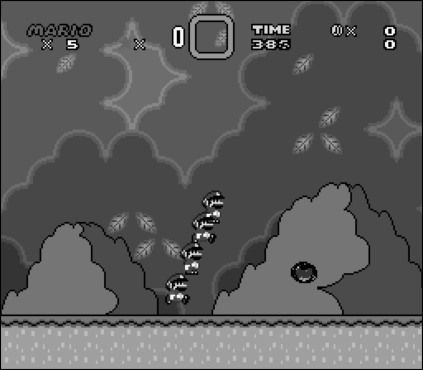
\includegraphics[width=.85\textwidth]{stacked}
    \end{figure}
    \subsection{Other}
    \subsubsection{Sticky Actions}
    \begin{itemize}
        \item AI needs to learn a policy that will work on other levels, not memorize one path in one level
        \item add stochasticity
        \item 25\% chance to repeat the previous action
    \end{itemize}
    \subsubsection{Episodic Life}
    \begin{itemize}
        \item Reset environment when a life is lost
        \item 5 lives, return to menu on death
        \item Prevent agent getting stuck in game menu
    \end{itemize}

    \section{Reward Shaping}
    \begin{itemize}
        \item ideal reward = +1 level complete (too sparse)
        \item end of level is always on the right side
        \item reward for moving right
        \item bonus for checkpoint/end of level
    \end{itemize}
    reward function based on https://github.com/Kautenja/gym-super-mario-bros/
    velocity: the difference in the agent's x position between states

    velocity = x1 - x0

    x0 is the x position before the step

    x1 is the x position after the step

    \begin{itemize}
        \item moving right $\Leftrightarrow$ $v > 0$
        \item moving left $\Leftrightarrow$ $v < 0$
        \item not moving $\Leftrightarrow$ $v = 0$
    \end{itemize}

    bonus:
    \begin{itemize}
        \item bonus of 'max reward'/2 for reaching checkpoint
        \item bonus of 'max reward' for reaching end of level
    \end{itemize}
    no penalty for death as this causes the agent to be too cautious (not enough exploration)

    total reward is clipped between 'min reward' and 'max reward' (default -15, 15)

    \section{Algorithm}
    \begin{itemize}
        \item Proximal Policy Optimization (PPO)
        \item Policy based algorithm
        \item Stable Baselines library\footnote{\url{https://github.com/DLR-RM/stable-baselines3}}
    \end{itemize}
    \subsection{Hyperparameters}
    \begin{itemize}
        \item learning\_rate = lambda $f$: $f * 1e^{-4}$
        \item n\_steps = 1024
        \item batch\_size = 512
        \item n\_epochs = 10
        \item gamma = 0.99
        \item gae\_lambda = 0.95
        \item clip\_range = 0.2
        \item ent\_coef = 0.01
        \item vf\_coef = 0.5
        \item max\_grad\_norm = 0.5
    \end{itemize}
    \section{Training \& Results}
    \subsection{Model A}
    Trained for 25 million time steps on the level 'YoshiIsland2'.
    Most basic level (avoid enemies, jump over pit).
    \begin{figure}[H]
        \centering
        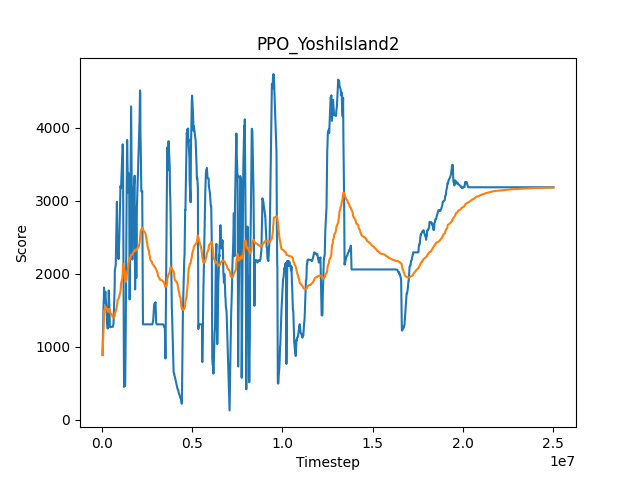
\includegraphics[width=\textwidth]{plot_model_a.png}
    \end{figure}
\end{document}